\documentclass[]{IEEEtran}

\title{Modellazione e Sintesi di un Moltiplicatore Floating-point Single Precision}
\author{Enrico Sgarbanti - VR446095}

\usepackage{graphicx}
\usepackage{wrapfig}
\usepackage{hyperref}
\usepackage[italian]{babel}
\usepackage[utf8]{inputenc}

\begin{document}
\maketitle


\begin{abstract}
    Questo documento mostra la realizzazione di un moltiplicatore in virgola mobile a precisione singola realizzato in VHDL, Verilog e SystemC ed un componente che permetta di eseguire due moltiplicazioni in parallelo. Il tutto è accompagnato da testbench, sintesi dei componenti VHDL e verilog ed un confronto con l'High-level-Synthesis di un moltiplicatore scritto in c++.
\end{abstract}


\section{Introduzione}
Il progetto consiste nella realizzaione in hardware di un sistema che esegue due moltiplicazioni in virgola mobile a precisione singola (quindi 32 bit) in parello secondo lo standard IEEE754. Esso deve essere sintetizzabile sulla scheda FPGA ``xc7z020clg400-1'' che possiede solo 125 porte, quindi si potranno avere a disposizione solo 64 bit per gli input e 32 per l'output. Di conseguenza bisogna serializzare input e output e usare il protocollo di handshake per gestire la comunicazione fra i vari componenti.
\\Il moltiplicatore sarà realizzato sia in Verilog che VHDL al fine di comprendere meglio le differenze e i pro e contro dei due linguaggi. L'intero sistema sarà poi tradotto anche in SystemC per fare un confronto anche con quel tipo di progettazione. Infine si analizzeranno i risultati e li si confronteranno con l'high level syntesis del codice in c++.
\\L'approccio utilizzato è bottom-up, cioè partendo dal moltiplicatore per poi arrivare al top level. L'implementazione è preceduta dall'analisi dei requisiti e la stesura della EFSM. La stesura dell'EFSM è la parte più importante perchè qui viene tradotto l'algoritmo, descritto il flusso e scelti i vari segnali e registri necessari. Una buona EFSM permette di evitare di scrivere varie righe di codice per poi accorgersi in simulazione che qualcosa non funziona.
\\Il progetto è piccolo quindi ci si aspetta che occupi una minima parte della FPGA e che la versione RTL sia 
\\Ci si aspetta che la versione RTL sia significativamente più performante di quella con l'high level syntesis, motivo per cui ha senso usare questo tipo di approccio quando non si hanno stretti vincoli di tempo da rispettare per realizzare il progetto.
\\Ci si aspetta anche che occupi una minima parte della FPGA in quanto è un progetto molto piccolo.


\section{Background}

\subsection{Progettazione hardware}
Per la realizzazione di componenti hardware si possono utilizzare diverse tecniche e linguaggi.
Un primo approccio è descrivere i componenti a livello RT utilizzando linguaggi di descrizione hardware (HDL) come VHDL e Verilog.
Un HDL è un linguaggio specializzato per la descrizione della struttura e del comportamento di circuiti elettronici, in particolare circuiti logici digitali, e la loro analisi e simulazione. Permette inoltre la sintesi di una descrizione HDL in una netlist (una specifica di componenti elettronici fisici e il modo in cui sono collegati insieme), che può quindi essere posizionata e instradata per produrre l'insieme di maschere utilizzate per creare un circuito integrato\cite{HDL}.
\\Un secondo approccio è descrivere le funzionalità del componente con linguaggi più ad alto livello come C, C++ o SystemC\cite{SystemC} e fare High Level Syntesis (HLS) per ottenere una descrizione dell'hardware a livello RT\cite{HLS}.
\\Entrambi gli approcci hanno vantaggi e svantaggi. In particolare HLS riduce i tempi, ma la descrizione hardware generata sarà meno ottimizzata rispetto a quella che si potrebbe ottenere usando HDL.


\subsection{IEEE 754 single-precision binary floating-point format}
Questo standard definisce il formato per la rappresentazione dei numeri in virgola mobile (compreso $\pm 0$ e i numeri denormalizzati; gli infiniti e i NaN, "not a number"), ed un set di operazioni effettuabili su questi. 
\\In particolare la versione a precisione singola descrive il numero con 32 bit: 1 bit per segno (sign), 8 bit per l'esponente (esp) e 23 bit per la mantissa (mant)\cite{IEEE754}.
\begin{figure}[!htb]
    \centering
    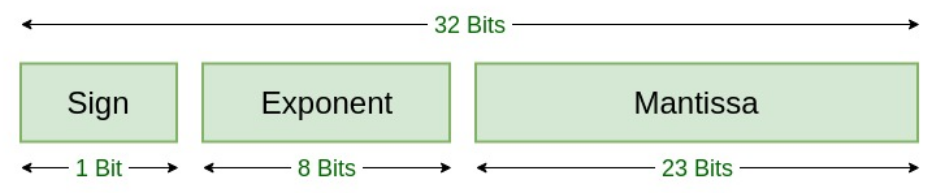
\includegraphics[width=0.9\linewidth]{figures/ieee754_single_precision.png}
    \caption{IEEE 754 single precision}
    \label{fig:IEEE754}
\end{figure}
\\Per la codifica in numero binario:
\begin{itemize}
    \item Dal segno si ricava il bit più significativo (1 se negativato 0 altrimenti).
    \item Si converte il numero in binario.
    \item Si sposta la virgola a sinistra fino ad avere un numero nella forma $1,... \cdot 2^{E}$.
    \item La mantissa è la parte a destra della virgola, riempita con zeri a destra fino a riempire i 23 bit.
    \item L'esponente è $127+E$ dove E è l'esponente ricavato dallo shift.
\end{itemize}
Per la decodifica del numero binario: $$(-1)^{sign}\cdot 2^{(esp-127)} \cdot (1 + \sum_{i=1}^{23}b_{23-i}\cdot 2^{-i})$$
\begin{figure}[!htb]
    \centering
    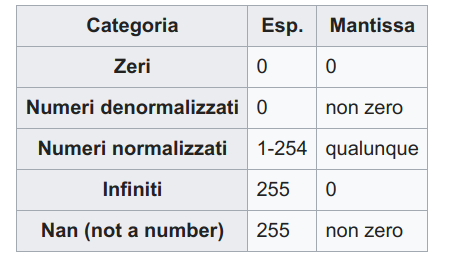
\includegraphics[width=0.6\linewidth]{figures/ieee754_special_case.png}
    \caption{IEEE 754 special case}
    \label{fig:IEEE_SPECIALCASE}
\end{figure}


\subsection{Moltiplicazione di due numeri floating-point}
Qui è riportato l'algoritmo usato per la moltiplicazione fra floating point. Guardare qui per ulteriori dettagli\cite{IEEE754Mult}.
\begin{figure}[!htb]
    \centering
    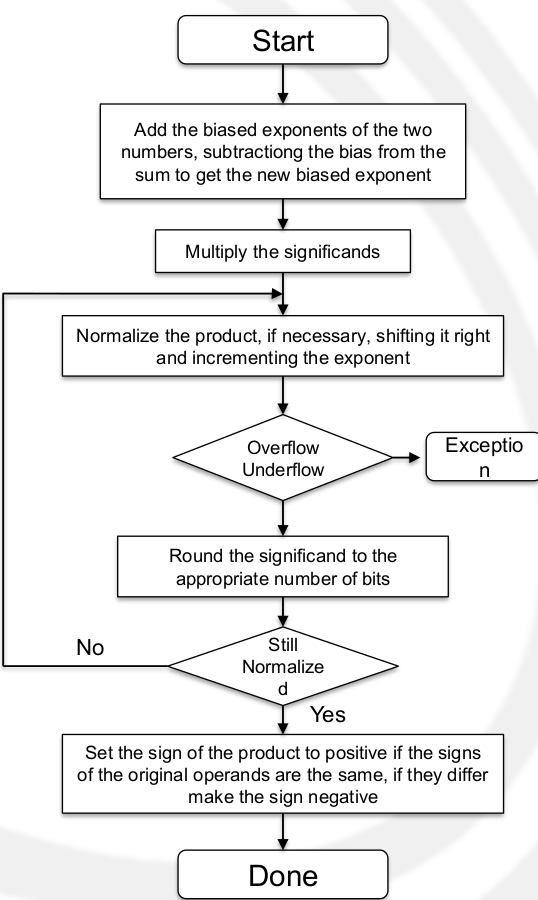
\includegraphics[width=0.6\linewidth]{figures/ieee_multiplication.png}
    \caption{IEEE 754 multiplication}
    \label{fig:IEEE_multiplication}
\end{figure}



\section{Metodologia applicata}
Il primo passo è stato la realizzazione della EFSM di \textit{multiplier} e \textit{double\_multiplier} che ha portato ad aquisire una visisione generale.
\\Dopo si è passati all'implementazione a livello RT con Vivado\cite{Vivado} del \textit{multiplier} sia in Verilog che in VHDL. Un primo test è stato fatto con TLC-script osservando gli output a determinati input.
\\Consolidati questi moduli è stato poi possibile realizzato in Verilog il \textit{double\_multiplier} che prende i due componenti e li usa per calcolare due moltiplicazioni. A questo punto è stato realizzato un test più accurato in verilog controllando tutti i casi particalari per poi passare alla sintesi.
\\È anche stato rifatto tutto in SystemC dove si è potuto fare un testbench più fine grazie alla potenza del c++.
\\Infine si è provato a fare l'high level syntesis da un semplice codice c++ per confrontare i risultati ottenuti.


\subsection{Vincoli ed Architettura}
Il progetto a diversi vincoli:
\begin{itemize}
    \item Il multiplier deve essere scritto in VHDL, verilog e systemC.
    \item Il double\_multiplier deve essere scritto in systemC e un linguaggio a scelta tra VHDL e verilog.
    \item Gli operandi e il risultato devono essere a 32 bit.
    \item I due componenti devono essere sintetizzabili sulla FPGA ``xc7z020clg400-1'' la quale ha a disposizione solo 125 porte.
\end{itemize}
Per far fronte al limite delle porte logiche è stato utilizzato il protocollo di handshake. Vengono quindi utilizzati gli stessi 32 bit per il risultato e altri 64 bit per le due coppie di operandi. Al primo ciclo di clock, con il flag ``ready'' uguale a 1, verranno trasmessi i primi due operandi e al ciclo successivo gli altri due. Dopodichè si aspetterà il complementanto delle moltiplicazioni, segnalato col flag ``done'' uguale a 1, per poi trasmettere il primo risultato, e il secondo al ciclo di clock successivo.
\\L'architettura con VHDL e Verilog è mostrata in figura \ref{fig:Architettura}. Quella per SystemC è analoga. 
\\I segnali intermedi sono stati omessi da questa figura, ma vengono descritti nelle sezioni successive.
\begin{figure}[!htb]
    \centering
    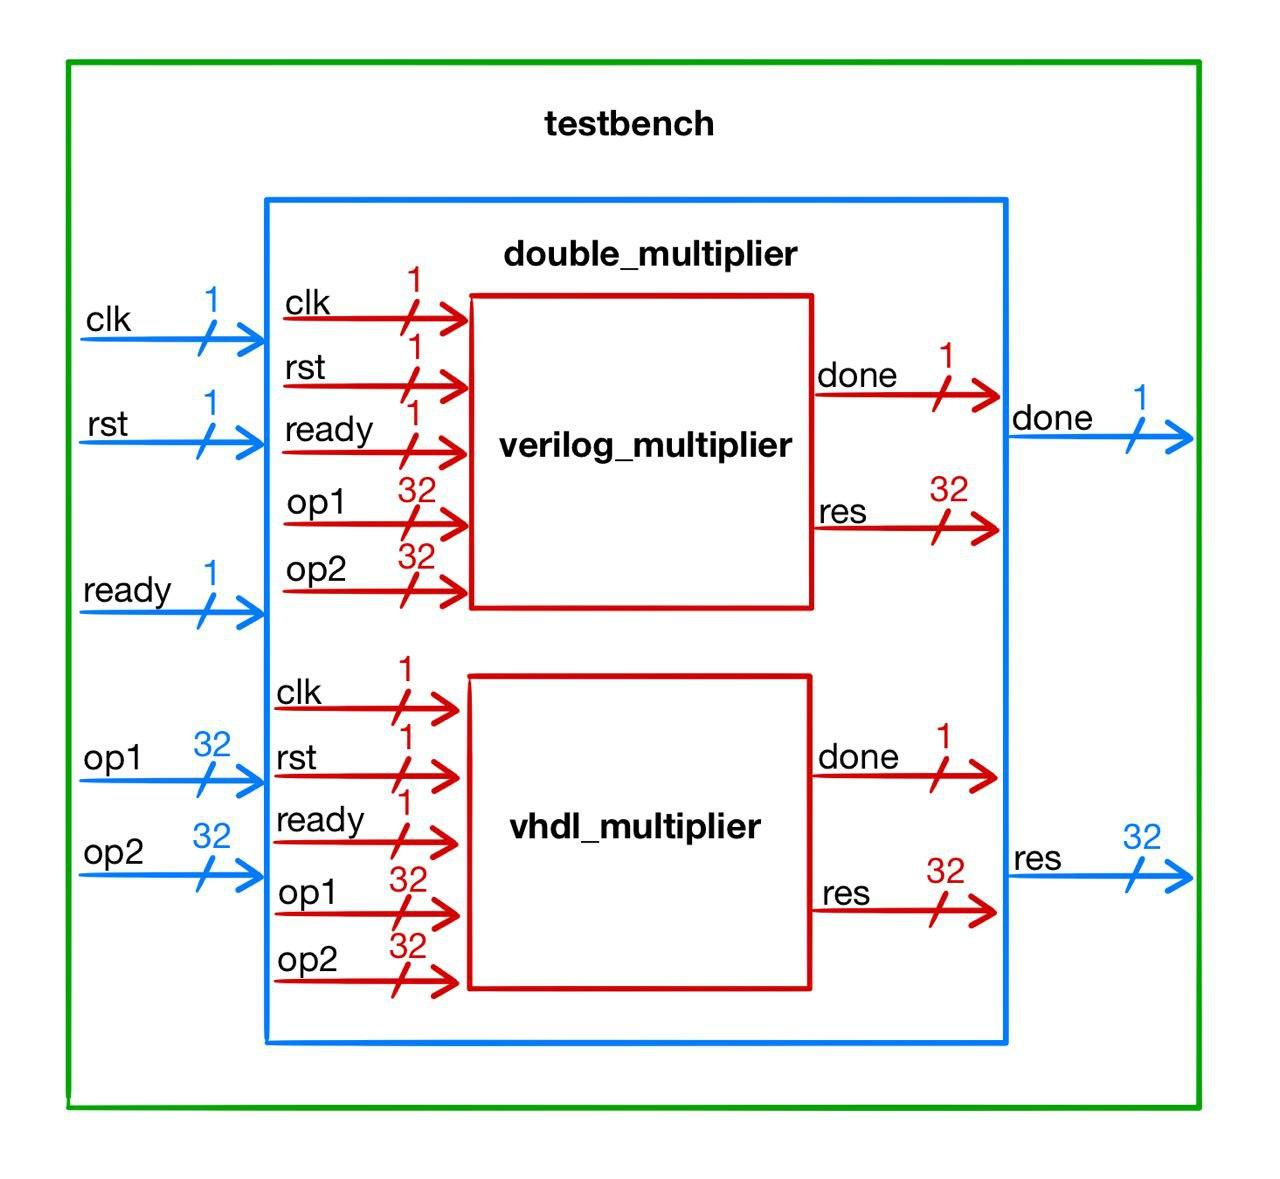
\includegraphics[width=0.8\linewidth]{figures/architettura.jpg}
    \caption{Architettura RTL}
    \label{fig:Architettura}
\end{figure}
La FSMD è realizzata con due processi:
\begin{itemize}
    \item \textbf{fsm:} processo asincrono attivato con la variazione di qualche segnale interno. Esso ha il compito di calcolare e aggiornare lo stato prossimo.
    \item \textbf{datapath:} processo sincrono che ha il compito di aggiornare lo stato attuale, elaborare gli output. Esso viene anche attivato dal fronte di salita del reset al fine di riportare lo stato a quello iniziale.
\end{itemize}


\subsection{multiplier}
Questo componente esegue la moltiplicazione tra numeri floating point a precisione singola.
\\L'interfaccia è mostrata in figura \ref{fig:Architettura} ed è la stessa per tutte le implementazioni VHDL, Verilog e SystemC: 
\begin{itemize}
    \item \textbf{op1} (32 bit input): primo operando.
    \item \textbf{op2} (32 bit input): secondo operando.
    \item \textbf{clk} (1 bit input): segnale di clock.
    \item \textbf{rst} (1 bit input): segnale di reset. Riporta il sistema allo stato iniziale.
    \item \textbf{ready} (1 bit input): segnale che permette al sistema di uscire dallo stato iniziale. Nello specifico indica che \textit{op1} e \textit{op2} contengono i valori dei due operatori.
    \item \textbf{done} (1 bit output): segnale che indica che il valore su \textit{res} è il risultato.
    \item \textbf{res} (32 bit output): risultato.
\end{itemize}
    
Gli altri segnali/registri intermedi utilizzati sono:
\begin{itemize}
    \item \textbf{norm\_again} (1 bit): indica che il numero ha bisogno di essere ulteriormente normalizzato.
    \item \textbf{res\_type} (2 bit): indicare il tipo del risultato. Solo nel caso in cui sia un numero si procede all'elaborazione, mentre negli altri casi si passa direttamente allo stato finale. Il caso del numero denormalizzato è gestito come se fosse normalizzato.
    \item \textbf{STATE e NEXT\_STATE} (4 bit): rappresentano lo stato attuale e lo stato prossimo.
    \item \textbf{op1\_type e op2\_type} (2 bit): per indicare il tipo degli operandi ovvero 0, NaN, $\infty$ oppure un numero. Solo se sono entrambi sono dei numeri res\_type sarà un numero.
    \item \textbf{esp\_tmp} (10 bit): permette di eseguire le operazioni per ricavare l'esponente finale senza perdere informazioni.
    \item \textbf{mant\_tmp} (48 bit): permette di eseguire le operazioni per ricavare la mantissa finale senza perdere informazioni.
    \item \textbf{sign1, sign2, esp1, esp2, mant1, mant2}: rappresentano le componenti dei due operandi.
\end{itemize}

L'algoritmo della moltiplicazione è descritto grazie alla EFSM [Figura \ref{fig:EFSM_multiplier}] la quale è formata 14 stati:
\begin{itemize}
    \item \textbf{ST\_START:} pone \textit{done} e \textit{norm\_again} a 0 ed estre le informazioni di segno, esponente e mantissa dei due operandi. Si rimane qui finchè \textit{ready} vale 0 altrimensi si passa a \textit{ST\_EVAL1}. Se in qualsiasi stato si riceve \textit{reset} uguale a 1 allora si passa a questo stato.
    \item \textbf{ST\_EVAL1 e ST\_EVAL2:} ricava rispettivamente il tipo di op1 e op2 fra \textit{T\_ZER, T\_INF, T\_NAN e T\_NUM}
    \item \textbf{ST\_EVAL3:} ricava il tipo del risultato in base al tipo di op1 e op2.
    \item \textbf{ST\_CHECK1:} controlla se \textit{res\_type} è uguale a T\_NUM e in tal caso passa a \textit{ST\_ELAB} altrimenti a \textit{ST\_FINISH}.
    \item \textbf{ST\_ELAB:} esegue la somma tra i due esponenti e la sottrazione di 127 in quanto entrambi, per lo standard, sono incrementati di 127: $(esp+127) = (esp1+127)+(esp2+127)-127$. Per compiere la somma è necessario usare una variabile \textit{esp\_tmp} di 10 bit perchè altrimenti con 8 bit si andrebbe in overflow con valori che dopo la sottrazione sarebbero rappresentabili con 8 bit e quindi validi. Viene poi eseguita anche la moltiplicazione delle due mantisse, che essendo a 23 bit più un bit che vale sempre 1, necessita di una variabile \textit{mant\_tmp} di almeno 48 bit
    \item \textbf{ST\_UNDERF:} controlla se \textit{esp\_tmp} è in uno stato di underflow, ovvero guardando se il bit \textit{esp\_tmp[9]}, che nel complemento a 2 indica il segno, è 1. Infatti i valori disponibili per l'esponente vanno da 0 a 255. Il controllo dell'overflow viene fatto in seguito all'arrotondamento per evitare di farlo due volte.
    \item \textbf{ST\_CHECK2:} passa allo stato \textit{ST\_FINISH} se \textit{res\_type} è diverso da \textit{T\_NUM}, perchè diventato \textit{T\_ZER} per l'underflow.
    \item \textbf{ST\_NORM1:} compie la normalizzazione della mantissa che deve sempre essere della forma \textit{1.bits}. Essendo la virgola posta tra il 46esimo bit e il 45esimo, si verificano due casi: Se il 47esimo bit vale 1 bisogna incrementare l'esponente, altrimenti il valore è già corretto, ma viene effettuato uno shift a sinistra per trattare allo stesso modo i due casi durante l'arrotondamento.
    \item \textbf{ST\_ROUND:} effettua l'eventuale arrotondamento dovuto al fatto che il valore della mantissa è attualmente a 48 bit, ma bisogna portarlo a 24 bit. L'arrotondamento è fatto per eccesso, quindi si incrementera \textit{mant\_tmp[47:24]} solo se \textit{mant\_tmp[23:00]} è $\geq$ a ``01..1''. L'arrotondamento effettivo verrà fatto nello stato \textit{ST\_NORM2}, qui ci si limita a porre \textit{norm\_again} uguale a 1 per poterci andare.
    \item \textit{\textbf{ST\_CHECK3:}} passa allo stato \textit{ST\_NORM2} se \textit{norm} è uguale a 1 oppure allo stato \textit{ST\_OVERF} se \textit{norm} è uguale a 0.
    \item \textbf{ST\_NORM2:} effettua il vero arrotondamento della mantissa. Bisogna tenere conto del caso in cui sia della forma ``1..1'' e che quindi con l'incremento vada a ``0..0'' e  venga incrementato l'esponente.
    \item \textbf{ST\_OVERF:} verifica se l'esponente del risultato è in uno stato di overflow, ovvero guardando se il bit \textit{esp\_tmp[8]} vale 1 ovvero se corrisponde ad un valore maggiore di 255.
    \item \textbf{ST\_FINISH:} pone \textit{done} uguale 1 e ricava \textit{res[31]}, ovvero il segno del risultato facendo lo XOR fra i segni degli operandi. In base al valore di \textit{res\_type} si ricavano gli altri bits e si torna allo stato iniziale.
\end{itemize}


\subsection{double\_multiplier}
Questo componente esegue due moltiplicazioni tra numeri floating point a precisione singola.
\\La scelta di realizzarlo in verilog è stata del tutto arbitraria.
\\L'interfaccia è mostrata in figura \ref{fig:Architettura} ed è la stessa sia per l'implementazione Verilog che quella SystemC:
\begin{itemize}
    \item \textbf{op1} (32 bit input): primo operando.
    \item \textbf{op2} (32 bit input): secondo operando.
    \item \textbf{clk} (1 bit input): segnale di clock.
    \item \textbf{rst} (1 bit input): segnale di reset. Riporta il sistema allo stato iniziale.
    \item \textbf{ready} (1 bit input): segnale che permette al sistema di uscire dallo stato iniziale. Nello specifico indica che in questo ciclo di clok \textit{op1} e \textit{op2} contengono gli operandi della prima moltiplicazione e nel ciclo di clock successivo ci saranno gli altri. (?)
    \item \textbf{done} (1 bit output): segnale che indica che il valore su \textit{res} è il risultato.
    \item \textbf{res} (32 bit output): risultato.
\end{itemize}
    
Gli altri segnali/registri intermedi utilizzati sono:
\begin{itemize}
    \item \textbf{ready1:} (1 bit) segnale che pone il \textit{ready} del primo multiplier (quello in Verilog) a 1.
    \item \textbf{ready2:} (1 bit) segnale che pone il \textit{ready} del secondo multiplier (quello in VHDL) a 1.
    \item \textbf{done1:} (1 bit) segnale che indica che il valore su \textit{res1} è il risultato della prima moltiplicazione.
    \item \textbf{done2:} (1 bit) segnale che indica che il valore su \textit{res2} è il risultato della seconda moltiplicazione.
    \item \textbf{op1\_tmp1, op2\_tmp1, op1\_tmp2, op2\_tmp2:} (32 bit) che servono a memorizzare temporaneamente gli operandi che arrivano nei vari cicli di clock. (?)
\end{itemize}

L'algoritmo è descritto grazie alla EFSM [Figura \ref{fig:EFSM_double_multiplier}] la quale è formata 8 stati:
\begin{itemize}
    \item \textbf{ST\_START:} pone \textit{done}, \textit{ready1} e \textit{ready2} uguali a 0 e inizializza \textit{op1\_tmp1} e \textit{op2\_tmp1} rispettivamenete con i valori di \textit{op1} e \textit{op2} i quali serviranno per il primo moltiplicatore. Si rimane qui finchè \textit{ready} vale 0 altrimensi si passa a \textit{ST\_RUN1}. Se in qualsiasi stato si riceve \textit{reset} uguale a 1 allora si passa a questo stato e si pone \textit{rst} uguale a 1 entrambi i \textit{rst} dei multiplier.
    \item \textbf{ST\_RUN1:} pone \textit{ready1} uguale a 1, attivando quindi il primo moltiplicatore, e inizializza \textit{op1\_tmp2} e \textit{op2\_tmp2} rispettivamenete con i valori di \textit{op1} e \textit{op2} i quali serviranno per il secondo moltiplicatore.
    \item \textbf{ST\_RUN2:} pone \textit{ready1} uguale a 0 e \textit{ready2} uguale a 1, attivando quindi il secondo moltiplicatore.
    \item \textbf{ST\_WAIT:} pone \textit{ready2} uguale a 0. Si rimane in questo stato finchè \textit{done1} $=1$ e in quel caso si passa a \textit{ST\_WAIT2} oppure che \textit{done2} $=1$ passando a {ST\_WAIT1}. Nel caso in cui sia \textit{done1} $=1$ che \textit{done2} $=1$ allora si passa direttamente a \textit{ST\_RET1}.
    \item \textbf{ST\_WAIT1:} si resta qui finchè non finisce anche il primo moltiplicatore, cioè finchè \textit{ready1} $=0$.
    \item \textbf{ST\_WAIT2:} si resta qui finchè non finisce anche il secondo moltiplicatore, cioè finchè \textit{ready2} $=0$.
    \item \textbf{ST\_RET1:} pone \textit{done} uguale a 1 e \textit{res} uguale al risultato del primo moltiplicatore cioè \textit{res1}.
    \item \textbf{ST\_RET2:} pone \textit{res} uguale al risultato del secondo moltiplicatore cioè \textit{res2} e ritorna allo stato iniziale.
\end{itemize}


\subsection{Implementazione RTL con Verilog e VHDL}
In \textbf{verilog\_multiplier} e \textit{double\_multiplier}
\begin{itemize}
    \item Sono definiti come ``wire'' tutti i segnali collegati alle porte di input mentre come ``reg'' tutti i registri collegati alle porte di output e quelli intermedi.
    \item Gli stati e \textit{op1\_type, op2\_type, res\_type} sono stati definiti come ``parameter''.
\end{itemize}
In \textbf{vhdl\_multiplier:}
\begin{itemize}
    \item Sono usate le librerie ``IEEE.STD\_LOGIC\_1164.ALL'' per abilitare i tipi std\_logic e ``use IEEE.NUMERIC\_STD.ALL'' per usare funzioni aritmetiche con valori signed e unsigned
    \item Sono definiti come ``signal'' tutti i segnali collegati alle porte di input e output.
    \item Sono definiti come ``signal'' tutti i segnali interni di communicazione per la FSM.
    \item Sono definite come ``variable'' \textit{sign1, sign2, esp1, esp2, esp\_tmp, mant1, mant2, mant\_tmp, op1\_type, op2\_type} perchè utilizzati solo all'interno del processo ``datapath''.
    \item Gli stati e \textit{op1\_type, op2\_type, res\_type} sono stati definiti all'interno del \textit{package} rispettivamente come ``MULT\_STATE'' e ``MULT\_TYPE''.
    \item L'architettura utilizzata segue lo stile ``behavioral'', cioè quello più ``program-like'' in quanto più semplice e chiaro per descrivere una FSMD con due processi.
\end{itemize}


\subsection{Implementazione RTL con SystemC}
Si creano i seguenti files e directory:
\begin{itemize}
    \item \textbf{Makefile:} tool per la compilazione automatica del progetto. Richiede che la variabile d'ambiente SYSTEMC\_HOME contenga il path alla libreria di SystemC.
    \item \textbf{bin:} directory che contiene l'eseguibile \textit{double\_multiplier\_RLT.x} (generato dopo la compilazione) e \textit{wave.vcd} (generato dopo l'esecuzione dell'eseguibile).
    \item \textbf{obj:} directory che contiene i files oggetto (generati dopo la compilazione)
    \item \textbf{include:} directory che contiene gli headers \textit{double\_multiplier\_RTL.hh}, \textit{multiplier\_RTL.hh}, \textit{testbench\_RTL.hh}. Qui sono definite tutte le porte, segnali, variabili ed enumerazioni dei vari componenti
    \item \textbf{testbench:} directory che contiene i files sorgenti \textit{double\_multiplier\_RTL.cc}, \textit{multiplier\_RTL.cc}, \textit{testbench\_RTL.cc} e \textit{main\_RTL.cc}.
\end{itemize}
In \textbf{double\_multiplier\_RTL.hh}
\begin{itemize}
    \item Sono definiti come ``sc\_signal'' tutti i segnali collegati alle porte di input e output.
    \item Sono definiti come ``sc\_signal'' tutti i segnali interni di communicazione per la FSM.
    \item Gli stati sono stati definiti come ``enumerazioni''.
\end{itemize}
In \textbf{multiplier\_RTL.hh}
\begin{itemize}
    \item Sono definiti come ``sc\_signal'' tutti i segnali collegati alle porte di input e output.
    \item Sono definiti come ``sc\_signal'' tutti i segnali interni di communicazione per la FSM.
    \item Sono definite come variabili di SystemC \textit{sign1, sign2, esp1, esp2, esp\_tmp, mant1, mant2, mant\_tmp, op1\_type, op2\_type} perchè utilizzati solo all'interno del processo ``datapath''.
    \item Gli stati e \textit{op1\_type, op2\_type, res\_type} sono stati definiti come ``enumerazioni''.
\end{itemize}
A differenza di verilog e VHDL, in SystemC è necessario un file ``main'' che contenga il metodo \textit{sc\_main} e che permetta di collegare il componente da testare con il testbench. In esso si utilizza \textit{sc\_create\_vcd\_trace\_file} per salvare le tracce necessarie a lanciare una simulazione con tools come gtkwave.


\section{Testbench}
Il \textbf{testbench in Verilog}, [Figura \ref{fig:SIM1}], aspetta un po di tempo, perchè altrimenti si verificherebbero problemi dovuti allo startup della FPGA nella simulazione post-sintesi, e poi esegue due volte il \textit{double\_multiplier}, prima con due coppie di operandi che danno come risultato dei numeri normali, e poi con due coppie di operandi che danno come risultati dei casi speciali. \\\\


Il \textbf{testbench in SystemC} mette a disposizione tre thread da attivare togliendo i commenti nel costruttore del ``TestbenchModule'':
\begin{itemize}
    \item \textbf{targeted\_test:} test analogo a quello in Verilog. [Figura \ref{fig:SIM2}].
    \item \textbf{rnd\_test:} test che prova \textit{TESTS\_NUM} moltiplicazioni generate casualmente tra un intervallo modificabile. [Figura \ref{fig:SIM3}].
    \item \textbf{run\_all:} che prova tutte le possibili combinazioni cioè \(2^{32} * 2^{32}\). Si può limitare il numero di combinazioni evitando di contare il bit del segno, in quanto il calcolo è un semplice xor. Poi si possono escludere tutti i numeri denormalizzati. In ogni caso risulta troppo pesante per essere eseguito.
\end{itemize}



\section{risultati}

\subsection{Simulazione Multiplier}
Per testare il corretto funzionamento di multiplier è stato usato lo script tlc mostrato in figura \ref{fig:SCRIPT}. Sono stati provati alcuni numeri a caso e i casi limite 0, NaN, $/infty$ e sono stati confrontati i valori finali e gli stati intermedi delle versioni in VHDL [Figura \ref{fig:SIM_MULT_VHDL}] e Verilog [Figura \ref{fig:SIM_MULT_VERILOG}] per garantirne la consistenza.
\\Per eseguire il multiplier bisogna attivare il reset e una volta che \textit{op1} e \textit{op2} contengono i valori si deve attiva anche il \textit{ready}. A questo punto il multiplier eseguira le elaborazioni indipendentemente dai valori di input, salvo per \textit{reset} che riperterà il tutto nello stato iniziale.


















\section{Conclusioni}


\bibliographystyle{IEEEtran}
\bibliography{biblio}
\appendix

\begin{figure*}[bt]
    \centering
    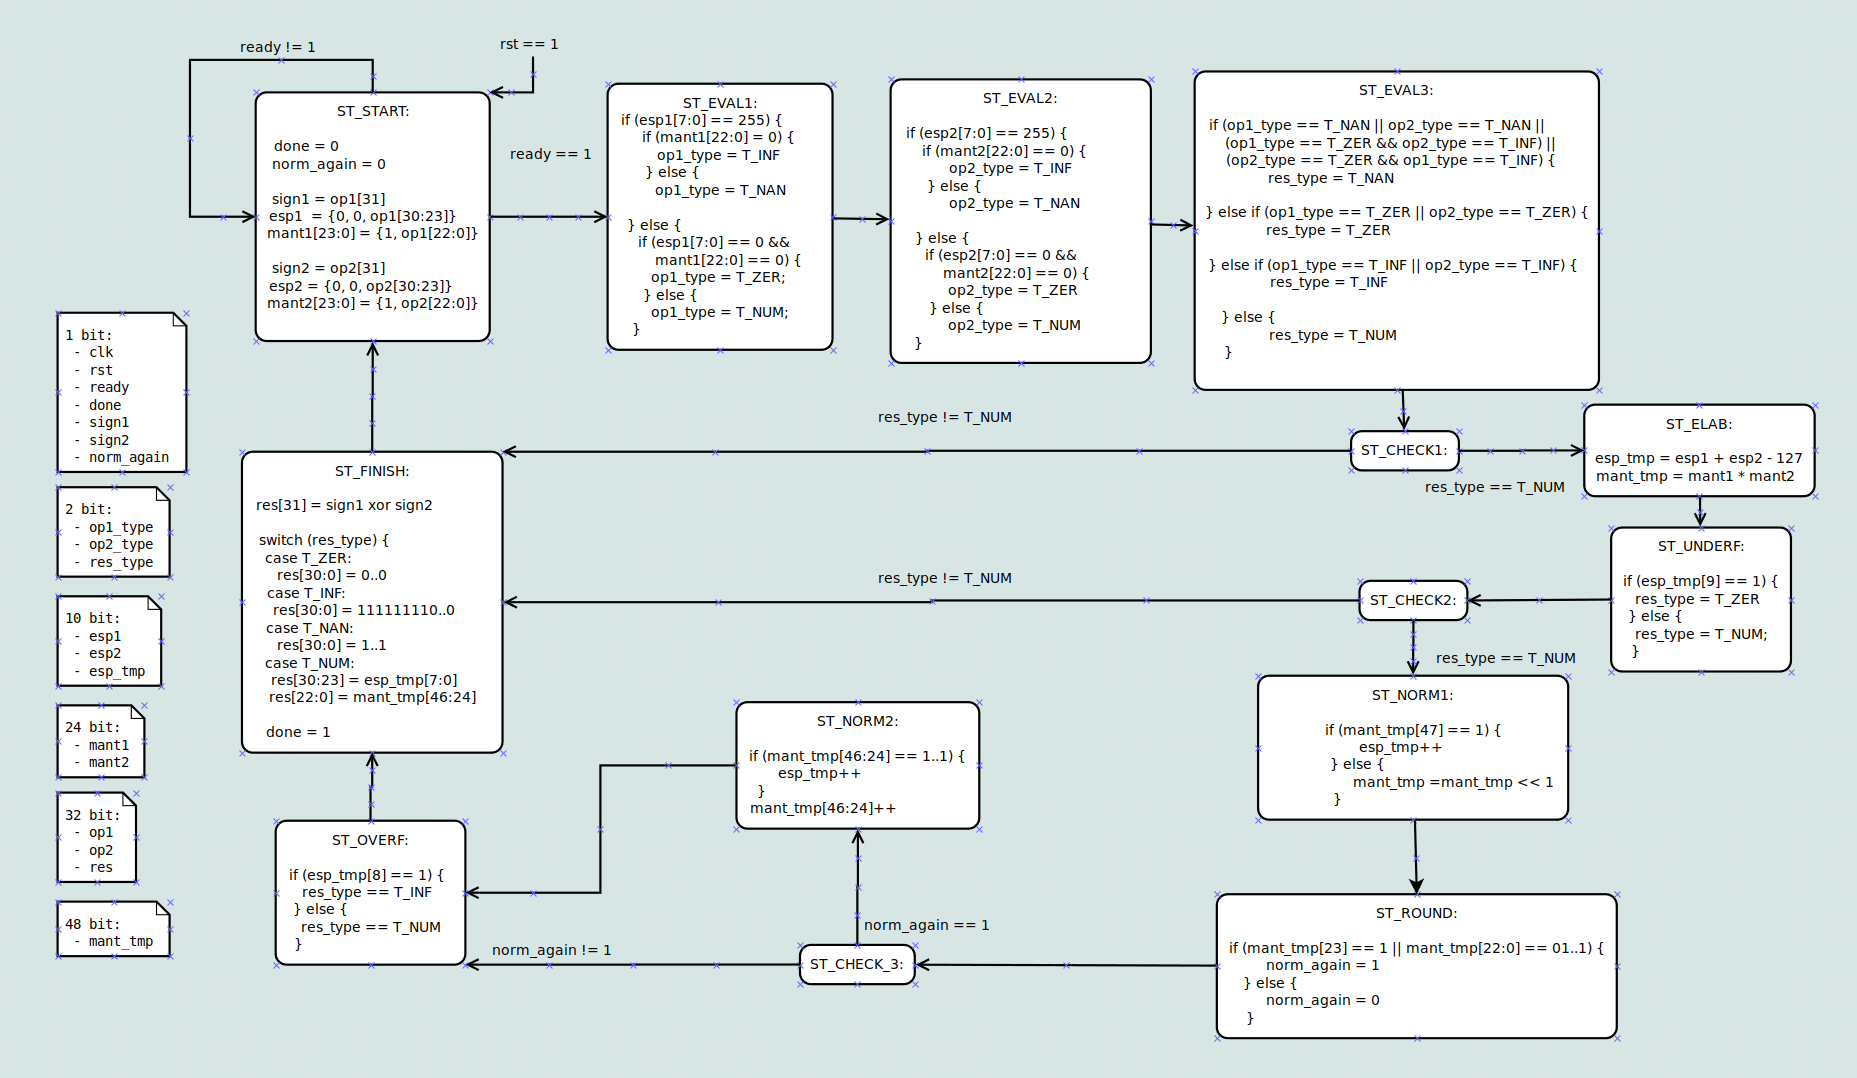
\includegraphics[width=\textwidth]{figures/EFSM-multiplier}
    \caption{EFSM del multiplier}
    \label{fig:EFSM_multiplier}
\end{figure*}

\begin{figure*}[bt]
    \centering
    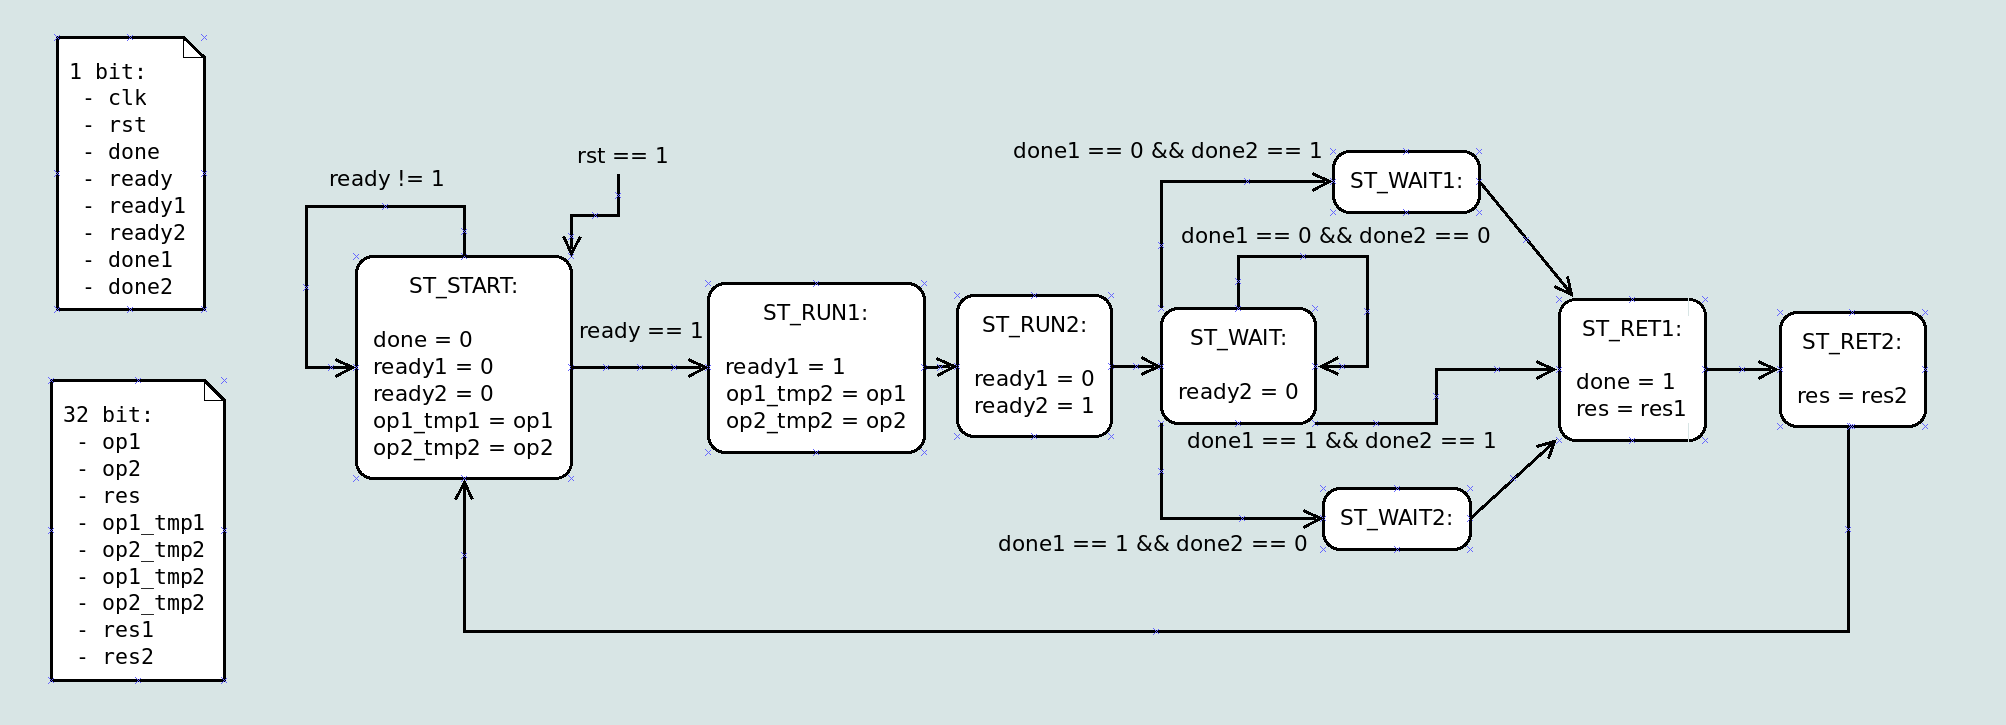
\includegraphics[width=\textwidth]{figures/EFSM-top_level}
    \caption{EFSM del double\_multiplier}
    \label{fig:EFSM_double_multiplier}
\end{figure*}


\begin{figure*}[bt]
    \centering
    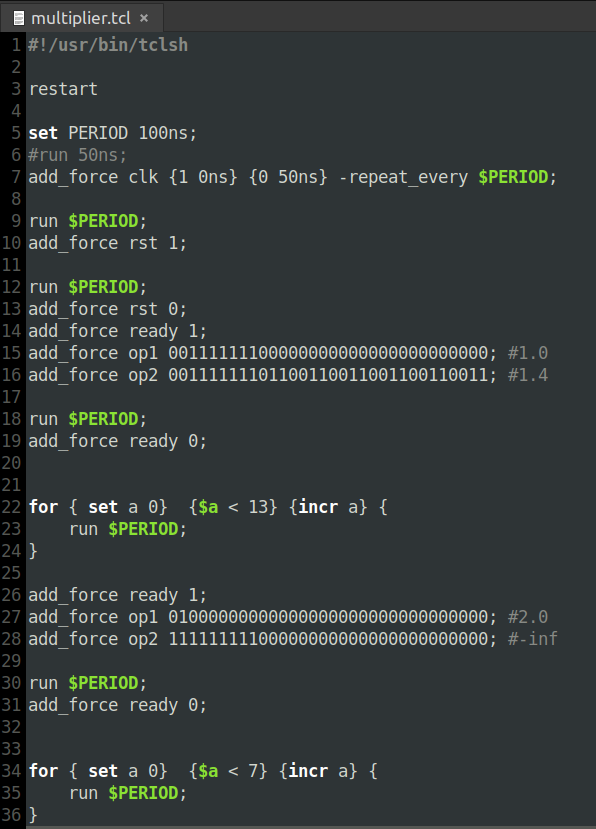
\includegraphics[width=0.4\textwidth]{figures/sim_mult_script}
    \caption{Script TLC utilizzato per il test del comportamento del multiplier}
    \label{fig:SCRIPT}
\end{figure*}

\begin{figure*}[bt]
    \centering
    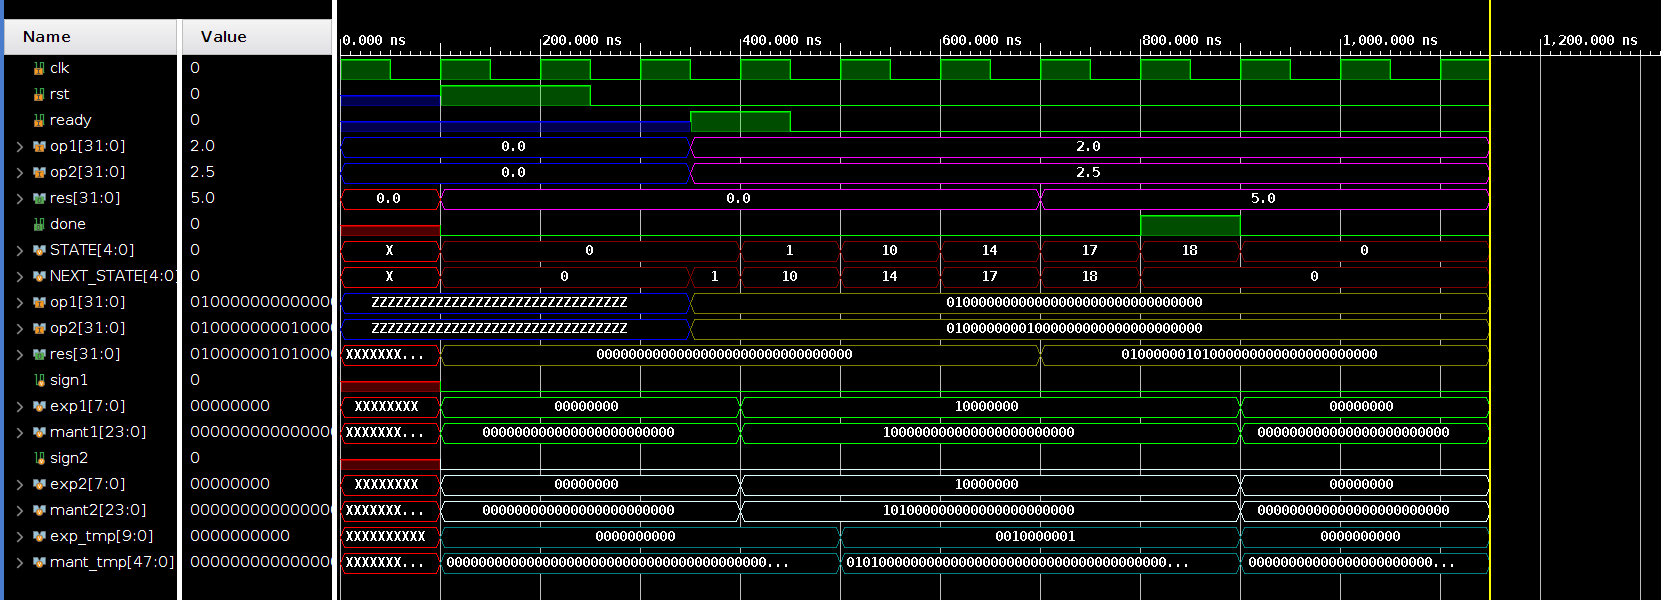
\includegraphics[width=\textwidth]{figures/sim_mult_verilog}
    \caption{Simulazione multiplier in VHDL con più zoom}
    \label{fig:SIM_MULT_VHDL_ZOOM}
\end{figure*}

\begin{figure*}[bt]
    \centering
    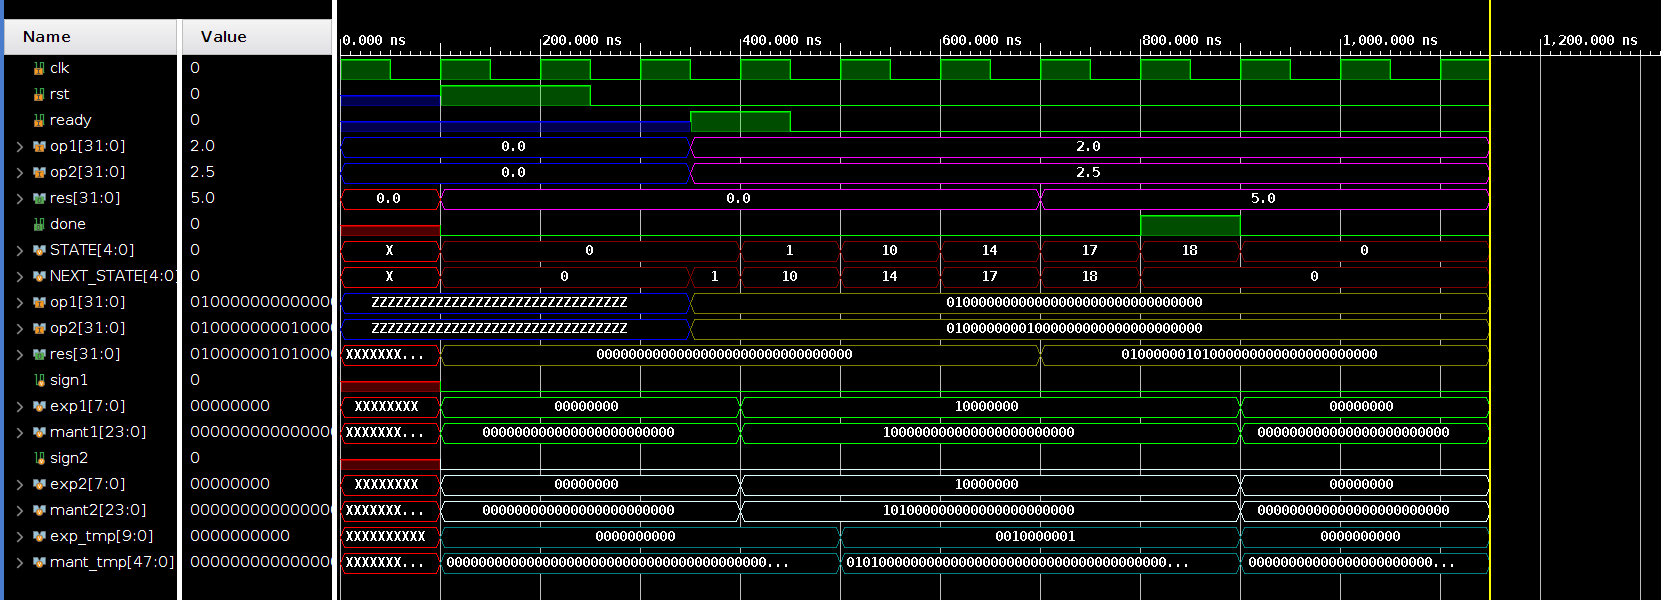
\includegraphics[width=\textwidth]{figures/sim_mult_verilog}
    \caption{Simulazione multiplier in VHDL}
    \label{fig:SIM_MULT_VHDL}
\end{figure*}

\begin{figure*}[bt]
    \centering
    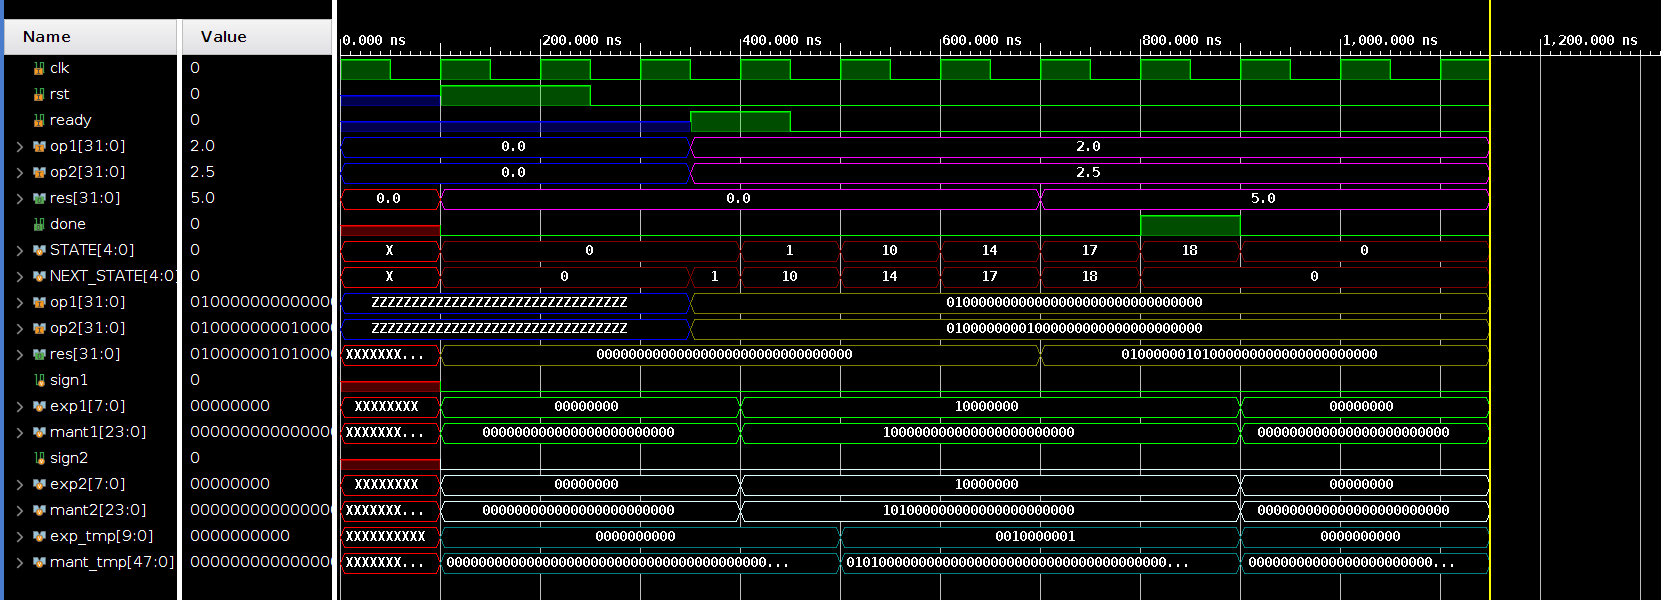
\includegraphics[width=\textwidth]{figures/sim_mult_verilog}
    \caption{Simulazione multiplier in Verilog}
    \label{fig:SIM_MULT_VERILOG}
\end{figure*}

















\begin{figure*}[bt]
    \centering
    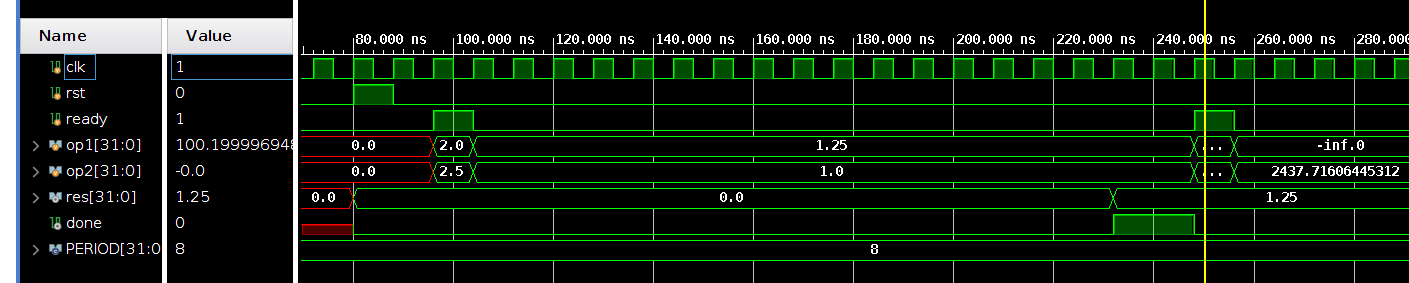
\includegraphics[width=\textwidth]{figures/simulazione1}
    \caption{Simulazione in Verilog}
    \label{fig:SIM1}
\end{figure*}

\begin{figure*}[bt]
    \centering
    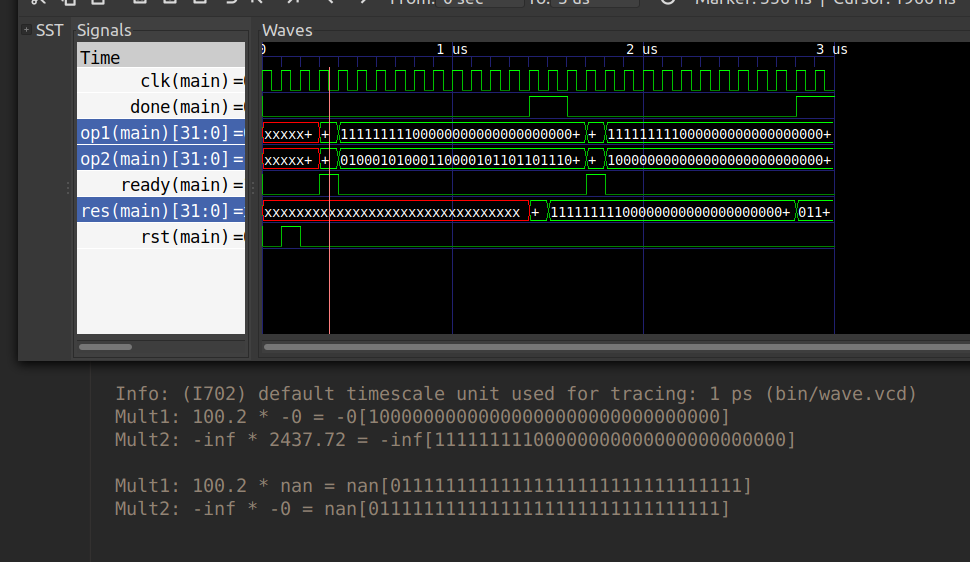
\includegraphics[width=\textwidth]{figures/simulazione2}
    \caption{Simulazione in SystemC con targeted\_test}
    \label{fig:SIM2}
\end{figure*}

\begin{figure*}[bt]
    \centering
    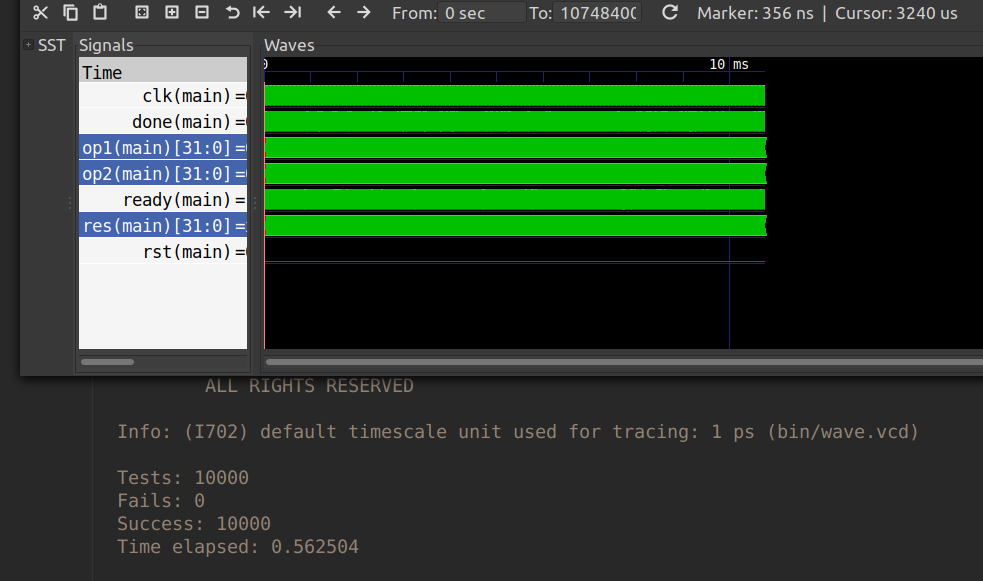
\includegraphics[width=\textwidth]{figures/simulazione3}
    \caption{Simulazione in SystemC con rnd\_test}
    \label{fig:SIM3}
\end{figure*}

\end{document}